\documentclass[notheorems,aspectratio=169]{beamer}
\usepackage{algorithm2e}

\usepackage{cmap}
\usepackage[T2A]{fontenc}
\usepackage[utf8]{inputenc}
\usepackage{mathtext}
\usepackage[english,russian]{babel}
\usepackage{commath}
\usepackage{gensymb}
\usepackage{amsfonts}
\usepackage{amssymb}
\usepackage{amsmath}
\usepackage{amsthm}
\usepackage{mathtools}
\usepackage{indentfirst}
\usepackage{geometry}
\usepackage{tikz}
\usepackage{tkz-euclide}
\usetkzobj{all}
\usetikzlibrary{arrows,positioning}
\usetikzlibrary{shapes,snakes}
\usetikzlibrary{shapes.multipart}
\usepackage{graphicx}
\usepackage{epstopdf}
\usepackage{subcaption}
\usepackage{caption}
\usepackage{hyperref}
\usepackage{setspace}
\usepackage{float}
\usepackage{tcolorbox}
\usepackage{totcount}
\usepackage{xcntperchap}
\captionsetup{justification=centering}
\usepackage{pgfpages}
\usepackage{pgfplots}
\usepackage{physics}
\usepackage{algorithm2e}
\usepackage{listings}

\mode<presentation>
{
	\usetheme{Warsaw}
	\usecolortheme{whale}
	\setbeamercovered{transparent}
	\useoutertheme{infolines}
}

\regtotcounter{section}
\regtotcounter{subsection}
\RegisterCounters{section}{subsection}


\newtheorem{theorem}{Theorem}
\newtheorem{example}{Example}
\newtheorem{definition}{Definition}
\DeclarePairedDelimiter\ceil{\lceil}{\rceil}
\DeclarePairedDelimiter\floor{\lfloor}{\rfloor}
\setbeamercovered{invisible}
\setbeamertemplate{navigation symbols}{}
\usepackage{physics}

\addtobeamertemplate{frametitle}{\setlength{\parindent}{0em}}{}
\addtobeamertemplate{block begin}{\setlength{\parindent}{0em}}{\setlength{\parindent}{2em}}
\addtobeamertemplate{block example begin}{\setlength{\parindent}{0em}}{\setlength{\parindent}{2em}}

\makeatletter
\setbeamertemplate{footline}
{
	\leavevmode%
	\hbox{%
		\begin{beamercolorbox}[wd=.5\paperwidth,ht=2.25ex,dp=1ex,center]{title in head/foot}%
			\usebeamerfont{title in head/foot}\insertshorttitle
		\end{beamercolorbox}%
		\begin{beamercolorbox}[wd=.42\paperwidth,ht=2.25ex,dp=1ex,center]{author in head/foot}%
			\usebeamerfont{author in head/foot}\insertshortauthor\beamer@ifempty{\insertshortinstitute}{}{, \insertshortinstitute}
		\end{beamercolorbox}%
		\begin{beamercolorbox}[wd=0.07\paperwidth,ht=2.25ex,dp=1ex,right]{date in head/foot}%
			\insertframenumber{} / \inserttotalframenumber\hspace*{2ex} 
		\end{beamercolorbox}}%
	\vskip0pt%
}

\setbeamertemplate{itemize items}[circle]
\setbeamertemplate{enumerate items}[circle]

\DeclareMathOperator*{\argmax}{arg\,max}
\DeclareMathOperator*{\argmin}{arg\,min}


\makeatletter
\title{Метод наименьших квадратов}
\author{Михаил Андреевич Терехов}
\institute[344 группа]{344 группа \\ Лаборатория распознавания изображений \\  СПбГУ}
\makeatletter
\subject{\@title}
\makeatother


\title{Метод наименьших квадратов}
\author{Михаил Андреевич Терехов}
\institute[344 группа]{344 группа \\ Лаборатория распознавания изображений \\  СПбГУ}
\date{2019}

\begin{document}
 
\begin{frame}
  \maketitle
  	\centering
\end{frame}

\begin{frame}
  \frametitle{Model fitting}

  \begin{columns}[b]
    \begin{column}{0.4\textwidth}
      \begin{figure}
        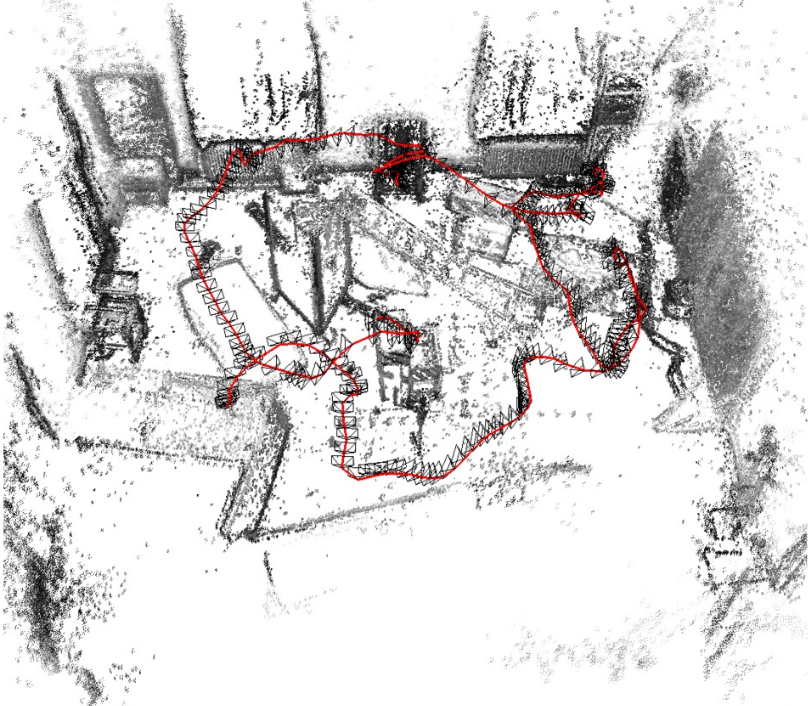
\includegraphics[width=0.5\linewidth, height=0.5\textheight, keepaspectratio]{vo.png}
        \caption*{Визуальная одометрия}
      \end{figure}
      \vspace{0pt}
    \end{column}

    \begin{column}{0.5\textwidth}
      \begin{figure}
        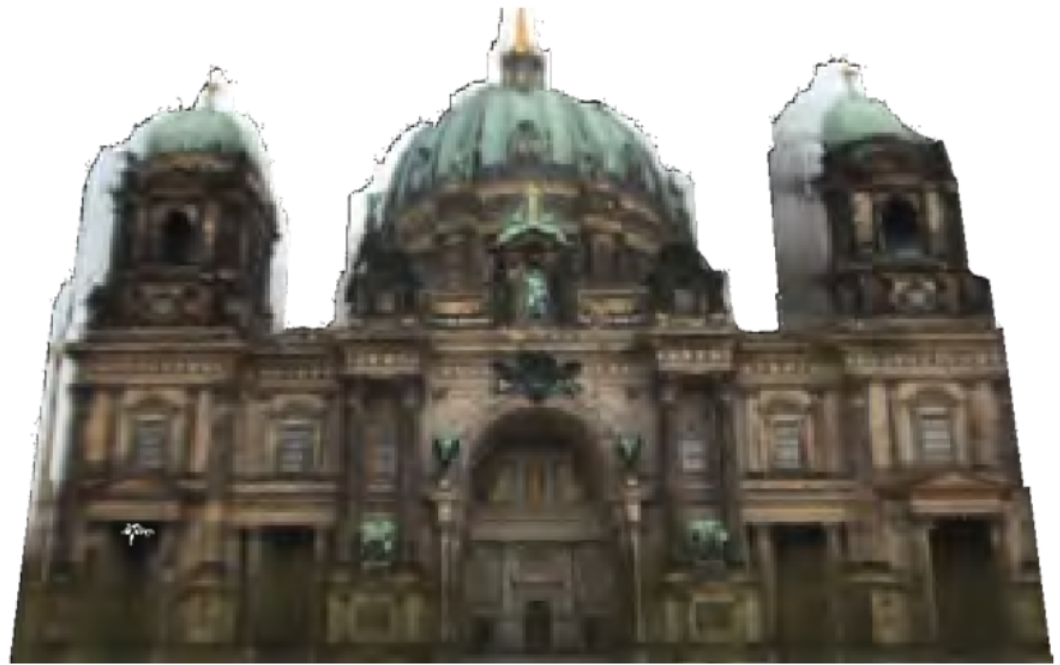
\includegraphics[width=0.5\linewidth, height=0.5\textheight, keepaspectratio]{berlin.png}
        \caption*{Трехмерные модели по набору фотографий}
      \end{figure}
      \vspace{0pt}
    \end{column}
  \end{columns}
 
  \begin{figure}
    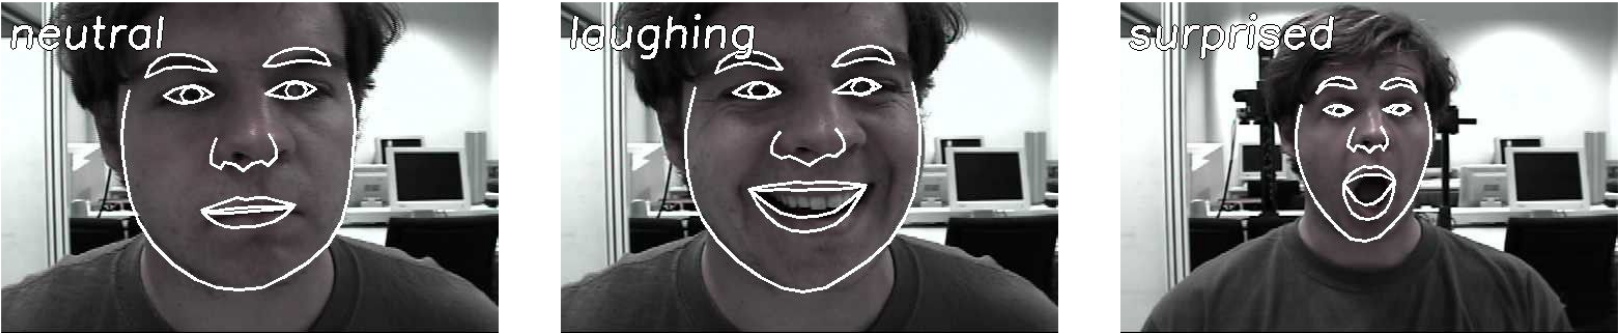
\includegraphics[width=0.5\linewidth, height=0.5\textheight, keepaspectratio]{emotions.png}
    \caption*{Определение эмоций по фотографии}
  \end{figure}

\end{frame}

\begin{frame}
  \frametitle{Постановка задачи}
  Возьмем сенсор (камеру, лидар, etc.). Пусть 
  \begin{itemize}
  \item $\mathbf{x}\in \mathbb{R}^m$ --- неизвестные параметры модели (положения точек, камер);
  \item $\left\{y_i: \mathbb{R}^m\to \mathbb{R}\right\}_{i=1}^n$ --- \emph{модель сенсора}, набор функций, сопоставляющих параметрам $\mathbf{x}$ ожидаемые данные $\left\{y_i\left(\mathbf{x}\right)\right\}$ (интенсивности, глубины); 
  \item $\left\{\tilde{y}_i\right\}$ --- набор реальных измерений;
  \item $\sigma_i$ --- качество $i$-го измерения.
  \end{itemize} 
  Тогда будем искать вектор $\mathbf{\tilde{x}}$, соответствующий модели, как
  \begin{equation*}
    \begin{gathered}
      \mathbf{\tilde{x}}=\argmin_{x\in \mathbb{R}^m}\sum_{i=1}^n \left(\frac{y_i\left(\mathbf{x}\right)-\tilde{y}_i}{\sigma_i}\right)^2 \\
    \end{gathered}
  \end{equation*}
\end{frame}

\begin{frame} 
  \frametitle{Функция остатков}
  Далее мы будем рассматривать более общую проблему вида
  \begin{equation*}
    \begin{gathered}
      \mathbf{r}: \mathbb{R}^m\to\mathbb{R}^n \\
      \mathbf{\tilde{x}}=\argmin_{x\in\mathbb{R}^m}\frac{1}{2}\left\Vert\mathbf{r}\left(\mathbf{x}\right)\right\Vert^2 \\
    \end{gathered}
  \end{equation*}
  $\mathbf{r}$ --- \emph{функция остатков}; $F\left(\mathbf{x}\right)=\frac{1}{2}\left\Vert\mathbf{r}\left(\mathbf{x}\right)\right\Vert^2$ --- \emph{целевая функция}.
  
  Нам также понадобится якобиан функции остатков
  $$\mathbf{J}=\dd{\mathbf{r}}$$
\end{frame}

\begin{frame}
  \frametitle{Предварительные подходы}
  \framesubtitle{Градиентный спуск}
  Запишем градиент целевой функции
  \begin{equation*}
    \begin{gathered}
      \mathbf{g}\left(\mathbf{x}\right)=\grad F\left(\mathbf{x}\right)=\mathbf{J}^\intercal \mathbf{r}\left(\mathbf{x}\right) \\
    \end{gathered}
  \end{equation*}
  
  Если совершать шаги вида $\mathbf{x}_{k+1}=\mathbf{x}_k-\frac{1}{\lambda}\mathbf{g}\left(\mathbf{x}_k\right)$ с достаточно большим $\lambda>0$, можно добиться убывания $\left\{F\left(\mathbf{x}_k\right)\right\}$. На практике такой подход не используется:
  \begin{itemize}
    \item маленькое $\lambda$ $\implies$ $F\left(\mathbf{x}_{k}+\Delta\mathbf{x}\right)\not\approx F\left(\mathbf{x}_k\right)-\grad F\left(\mathbf{x}_k\right)^\intercal\Delta\mathbf{x}$
    \item большое $\lambda$ $\implies$ медленная сходимость
  \end{itemize}
\end{frame}

\begin{frame}
  \frametitle{Предварительные подходы}
  \framesubtitle{Метод Гаусса-Ньютона}
  Можно линеаризовать не целевую функцию, а функцию остатков
  \begin{equation*}
    \begin{gathered}
      \mathbf{r}\left(\mathbf{x}+\Delta\mathbf{x}\right)\approx\mathbf{r}\left(\mathbf{x}\right)+\mathbf{J}\Delta\mathbf{x} \\
      F\left(\mathbf{x}+\Delta\mathbf{x}\right)\approx\frac{1}{2}\left\Vert\mathbf{r}\left(\mathbf{x}\right)\right\Vert^2+\left(\mathbf{J}^\intercal\mathbf{r}\left(\mathbf{x}\right)\right)^\intercal\Delta\mathbf{x}+\frac{1}{2}\Delta\mathbf{x}^\intercal\mathbf{J}^\intercal\mathbf{J}\Delta\mathbf{x}\\
    \end{gathered}
  \end{equation*}
  Вспомним, что $\mathbf{J}^\intercal\mathbf{r}\left(\mathbf{x}\right)=\mathbf{g}$, и положим $\mathbf{H}=\mathbf{J}^\intercal\mathbf{J}$
  \begin{equation*}
    \begin{gathered}
      F\left(\mathbf{x}+\Delta\mathbf{x}\right)\approx\frac{1}{2}\left\Vert\mathbf{r}\left(\mathbf{x}\right)\right\Vert^2+\mathbf{g}^\intercal\Delta\mathbf{x}+\frac{1}{2}\Delta\mathbf{x}^\intercal\mathbf{H}\Delta\mathbf{x}\\
    \end{gathered}
  \end{equation*}
\end{frame}

\begin{frame}
  \frametitle{Предварительные подходы}
  \framesubtitle{Метод Гаусса-Ньютона}
  Теперь в качестве шага можно выбирать минимум полученного приближения $F$\footnote[frame]{Предполагаем $n\geq m$, и что $\mathbf{J}$ --- полного ранга.}
  \begin{align*}
    \Delta\mathbf{x}_k & =\argmin_{\Delta\mathbf{x}\in \mathbb{R}^m}\frac{1}{2}\left\Vert\mathbf{r}+\mathbf{J}\Delta\mathbf{x}\right\Vert^2 \\
                       & =\argmin_{\Delta\mathbf{x}\in \mathbb{R}^m}\left(\mathbf{g}^\intercal\Delta\mathbf{x}+\frac{1}{2}\Delta\mathbf{x}^\intercal\mathbf{H}\Delta\mathbf{x}\right)=\mathbf{H}^{-1}\mathbf{g} \\
      \mathbf{x}_{k+1}=\mathbf{x}_k+\Delta\mathbf{x}_k \\
  \end{align*}

    Более точное приближение целевой функции $\implies$ точные крупные шаги.

    Но что делать, если шаг всё-таки неудачный?
\end{frame}

\begin{frame}
  \frametitle{Алгоритм Левенберга-Марквардта}
  \framesubtitle{Интуитивное описание}
  В случае, если шаг Гаусса-Ньютона оказывается неудачным, можно ``подправить'' его так, чтобы он стал больше похож на шаг градиентного спуска
  \begin{equation*}
    \begin{gathered}
      \Delta\mathbf{x}_k=-\left(\mathbf{H}+\lambda\mathbf{I}\right)^{-1}\mathbf{g} \\
    \end{gathered}
  \end{equation*}

  Если $\Delta\mathbf{x}_k$ оказалось неудачным, увеличим $\lambda$ и попробуем ещё раз.
  
  При $\lambda\rightarrow\infty$ $\Delta\mathbf{x}\approx -\frac{1}{\lambda}\mathbf{g}$ $\implies$ можем сделать удачный шаг при достаточно большом $\lambda$.

\end{frame}

\begin{frame}
  \frametitle{Алгоритм Левенберга-Марквардта}
  \framesubtitle{Как метод доверительного региона}
  Будем считать, что оценка $\mathbf{r}\left(\mathbf{x}+\Delta\mathbf{x}\right)\approx\mathbf{r}\left(\mathbf{x}\right)+\mathbf{J}\Delta\mathbf{x}$ выполнена при $\left\Vert\Delta\mathbf{x}\right\Vert<\mu$. Тогда очередной шаг алгоритма имеет смысл выбирать как
  \begin{equation*}
    \begin{gathered}
      \Delta\mathbf{x}_{nice}=\argmin_{\left\Vert\Delta\mathbf{x}\right\Vert\leq\mu}\left(\mathbf{g}^\intercal\Delta\mathbf{x}+\frac{1}{2}\Delta\mathbf{x}^\intercal\mathbf{H}\Delta\mathbf{x}\right)
    \end{gathered}
  \end{equation*}

  Оказывается, что
  \begin{itemize}
    \item $\left\Vert\Delta\mathbf{x}_{nice}\right\Vert<\mu \implies \Delta\mathbf{x}_{nice}=-\mathbf{H}^{-1}\mathbf{g}$
    \item $\left\Vert\Delta\mathbf{x}_{nice}\right\Vert=\mu \implies \exists\lambda: \Delta\mathbf{x}_{nice}=-\left(\mathbf{H}+\lambda\mathbf{I}\right)^{-1}\mathbf{g}$
  \end{itemize}
  
\end{frame}

\begin{frame}
  \frametitle{Алгоритм Левенберга-Марквардта}
  \framesubtitle{Как метод доверительного региона}
  И в обратную сторону, если мы выбрали $\Delta\mathbf{x}_k$ согласно алгоритму
  \begin{equation*}
    \begin{gathered}
      \Delta\mathbf{x}_k=-\left(\mathbf{H}+\lambda\mathbf{I}\right)^{-1}\mathbf{g} \\
    \end{gathered}
  \end{equation*}
  и положили $\mu=\left\Vert\Delta\mathbf{x}_k\right\Vert$, то 

  \begin{equation*}
    \Delta\mathbf{x}_k=\argmin_{\left\Vert\Delta\mathbf{x}\right\Vert\leq\mu}\left(\mathbf{g}^\intercal\Delta\mathbf{x}+\frac{1}{2}\Delta\mathbf{x}^\intercal\mathbf{H}\Delta\mathbf{x}\right)
    \end{equation*}

    Если мы знаем $\mu$, то нам неизвестен $\lambda$, который нужно использовать, чтобы попасть точно на границу. Но мы можем воспользоваться эвристикой $\lambda\approx\frac{1}{\mu}$.
\end{frame}

\begin{frame}
  \frametitle{Алгоритм Левенберга-Марквардта}
  \framesubtitle{Как метод доверительного региона}
  После того, как мы сделали очередной шаг $\Delta\mathbf{x}_k$, мы можем оценить качество модели. Обычно для этого используется отношение реального изменения целевой функции к предсказанному
  \begin{equation*}
    \rho=\frac{F\left(\mathbf{x}_k\right)-F\left(\mathbf{x}_k+\Delta\mathbf{x}\right)}{F\left(\mathbf{x}_k\right)-\frac{1}{2}\left\Vert\mathbf{r}\left(\mathbf{x}_k\right)+\mathbf{J}\Delta\mathbf{x}\right\Vert^2}
  \end{equation*}

  Если $\rho$ особенно ``плохое'' (несколько порядков), то шаг отбрасыватся. Иначе шаг происходит, и в зависимости от $\rho$ доверительный регион либо увеличивается, либо уменьшается.
\end{frame}

\begin{frame}
  \frametitle{Алгоритм Левенберга-Марквардта}
  \framesubtitle{Резюме}

\begin{algorithm}[H]
  \SetAlgoLined
  Выбираем $\mathbf{x}_0$ и $\mu_0$, $k=0$\;
  \While{Не выполнены критерии остановки}
  {
    $\Delta\mathbf{x}_k=-\left(\mathbf{H}+\frac{1}{\mu_k}\mathbf{I}\right)^{-1}\mathbf{g}$\;
    Рассчитываем $\rho$ для шага $\Delta\mathbf{x}_k$\;
    \uIf{$\rho<\rho_{crit}$}
    {
      $\mathbf{x}_{k+1}=\mathbf{x}_k$; \quad $\mu_{k+1}=\frac{\mu_k}{2}$\;
    }
    \uElseIf{$\rho<\rho_{bad}$}
    {
      $\mathbf{x}_{k+1}=\mathbf{x}_k+\Delta\mathbf{x}_k$; $\quad \mu_{k+1}=\frac{\mu_k}{2}$\;
    }
    \uElseIf{$\rho\approx 1$}
    {
      $\mathbf{x}_{k+1}=\mathbf{x}_k+\Delta\mathbf{x}_k$; \quad $\mu_{k+1}=2\mu_k$\;
    }
    \Else
    {
      $\mathbf{x}_{k+1}=\mathbf{x}_k+\Delta\mathbf{x}_k$; \quad $\mu_{k+1}=\mu_k$\;
    }
  }
\end{algorithm}

\end{frame}

\begin{frame}
  \frametitle{Дифференцирование}
  Существуют 3 основных способа вычислять производные:
  \begin{itemize}
    \item Символьно
    \item Численно
    \item Автоматически
  \end{itemize}
\end{frame}

\begin{frame}
  \frametitle{Дифференцирование}
  \framesubtitle{Численные методы}
  Пусть $f$ --- исследуемая функция. Распишем её ряд Тейлора
  \begin{equation*}
    \begin{gathered}
      f\left(x+h\right)=f\left(x\right)+f'\left(x\right)h+f^{(2)}\left(x\right)\frac{h^2}{2}+O\left(h^3\right) \\
      f\left(x-h\right)=f\left(x\right)-f'\left(x\right)h+f^{(2)}\left(x\right)\frac{h^2}{2}+O\left(h^3\right) \\
    \end{gathered}
  \end{equation*}

  \begin{itemize}
    \item Метод односторонней разности
      \begin{equation*}
        f'\left(x\right)=\frac{f\left(x+h\right)-f\left(x\right)}{h}+O\left(h\right)
      \end{equation*}
    \item Метод симметричной разности 
      \begin{equation*}
        f'\left(x\right)=\frac{f\left(x+h\right)-f\left(x-h\right)}{2h}+O\left(h^2\right)
      \end{equation*}
  \end{itemize}
\end{frame}

\begin{frame}
  \frametitle{Дифференцирование}
  \framesubtitle{Метод Риддера}
  Положим 
  \begin{equation*}
    \begin{gathered}
      A\left(1, m\right)=\frac{f\left(x+h/2^{m-1}\right)-f\left(x-h/2^{m-1}\right)}{2h/2^{m-1}} \\
      A\left(n+1, m\right)=\frac{4^{n-1}A\left(n,m+1\right)-A\left(n,m\right)}{4^{n-1}-1} \\
    \end{gathered}
  \end{equation*}
  \vspace{1cm}
  \begin{columns}[c]
    \begin{column}{0.5\textwidth}
      Оказывается, что $f'\left(x\right)=A\left(n,1\right)+O\left(h^{2n}\right)$
    \end{column}
    \begin{column}{0.5\textwidth}
      $$
      \begin{matrix}
        A\left(1,1\right) & A\left(1,2\right) & A\left(1,3\right) & A\left(1,4\right) \\
                          & A\left(2,1\right) & A\left(2,2\right) & A\left(2,3\right) \\
                          &                   & A\left(3,1\right) & A\left(3,2\right) \\
                          &                   &                   & A\left(4,1\right) \\
      \end{matrix}
      $$
    \end{column}
  \end{columns}
\end{frame}

\begin{frame}
  \frametitle{Дифференцирование}
  \framesubtitle{Численные методы, выбор шага}
  Рассмотрим функцию $f\left(x\right)=\sqrt{x}\sin\left(\frac{1}{x}\right)$, $x_0=0.1$. Будем искать $f'\left(x_0\right)$.
  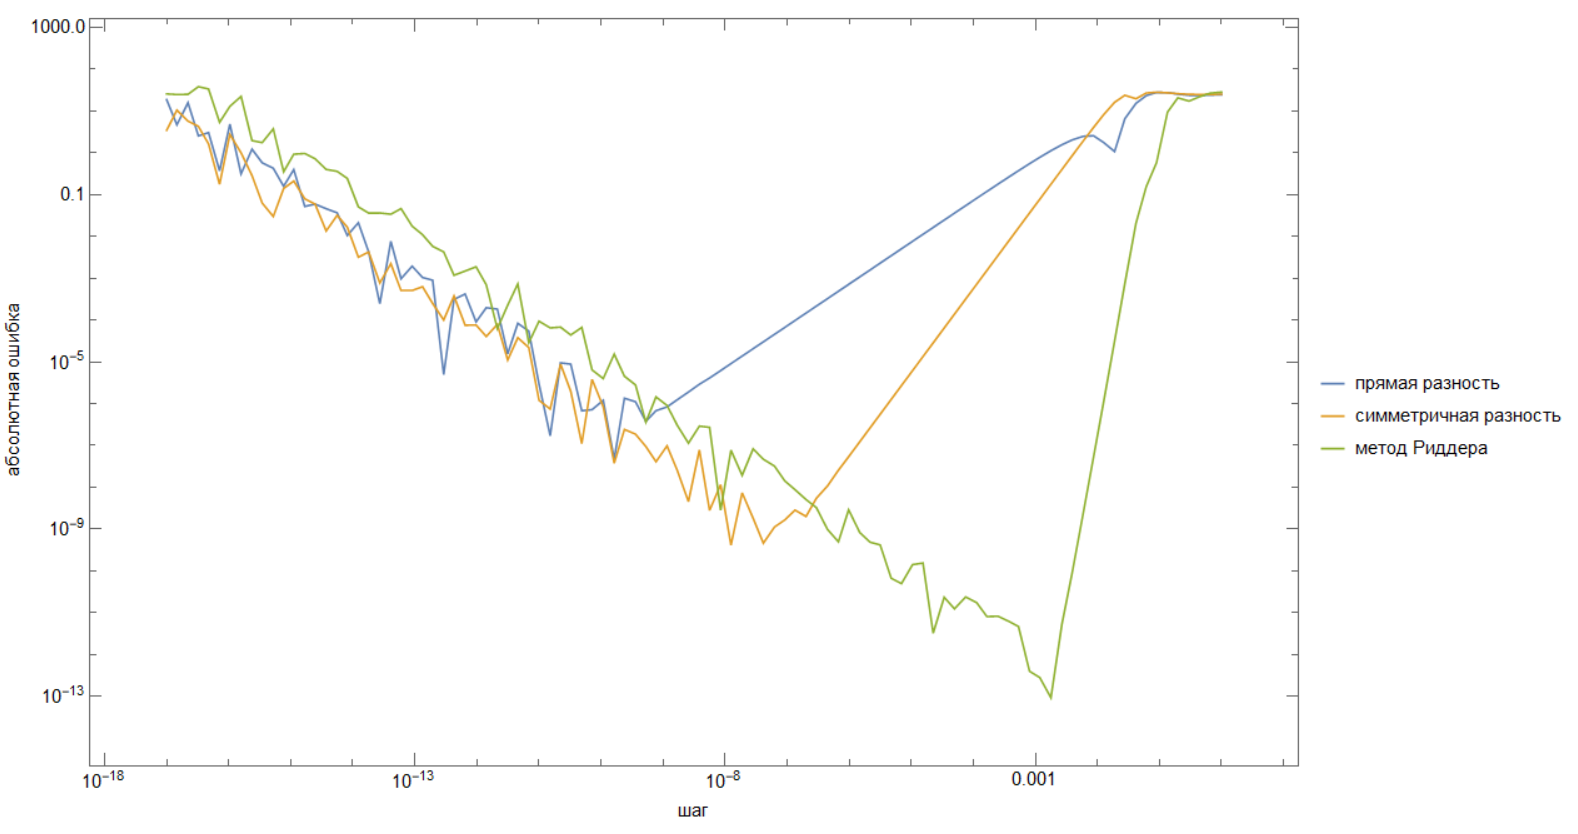
\includegraphics[height=0.65\textheight, keepaspectratio]{diff-err.png}
\end{frame}

\begin{frame}
  \frametitle{Дифференцирование}
  \framesubtitle{Автоматическое дифференцирование, дуальные числа}

  Введем абстрактный элемент $\varepsilon$ (\emph{инфинитезималь}) такой, что $\varepsilon^2=0$. Будем рассматривать числа вида $a+b\varepsilon$. 
  \begin{itemize}
    \item $\left(a_1+b_1\varepsilon\right)\pm\left(a_2+b_2\varepsilon\right)=\left(a_1\pm a_2\right)+\left(b_1\pm b_2\right)\varepsilon$
    \item $\left(a_1+b_1\varepsilon\right)\left(a_2+b_2\varepsilon\right)=a_1a_2+\left(a_1b_2+a_2b_1\right)\varepsilon$
    \item $\frac{a_1+b_1\varepsilon}{a_2+b_2\varepsilon}=\frac{a_1}{a_2}+\frac{a_1b_2-a_2b_1}{a_2^2}\varepsilon$
  \end{itemize}
  Более того, если $f\left(x+h\right)=f\left(x\right)+f'\left(x\right)h+o(h)$, то
  $$f\left(x+b\varepsilon\right)=f\left(x\right)+bf'\left(x\right)\varepsilon$$
  Значит, если мы научимся производить вычисления с дуальными числами, мы получим способ вычислять производную по ходу вычисления функции!
\end{frame}

\begin{frame}
  \frametitle{Дифференцирование}
  \framesubtitle{Автоматическое дифференцирование, дуальные числа}
  Введем теперь дуальные числа вида $a+\mathbf{v}$ с $m$-мерной инфинитезимальной компонентой.

  Если $f: \mathbb{R}^m\to\mathbb{R}$, то положим 
  $$f\left(a_1+\mathbf{v}_1,\dotsc,a_m+\mathbf{v}_m\right)=f\left(a_1,\dotsc,a_m\right)+V\grad f$$
  где $\left\{\mathbf{v}_i\right\}$ --- столбцы $V_{m\cross m}$

  Если $\mathbf{g}:\mathbb{R}^m\to\mathbb{R}^n$, то якобиан $\mathbf{J_g}$ функции $\mathbf{g}$ в точке $\mathbf{x}$ можно вычислить так 
  \begin{equation*}
    \begin{gathered}
      \mathbf{g}\left(x_1+\mathbf{e}_1,\dotsc,x_m+\mathbf{e}_m\right)=
      \begin{pmatrix}
        g_1\left(\mathbf{x}\right)+\mathbf{u}_1 \\
        \vdots \\
        g_n\left(\mathbf{x}\right)+\mathbf{u}_n \\
      \end{pmatrix} \\
      \mathbf{J_g}=
      \begin{pmatrix}
        \mathbf{u}_1^\intercal \\
        \vdots \\
        \mathbf{u}_n^\intercal \\
      \end{pmatrix}
    \end{gathered}
  \end{equation*}

\end{frame}

\begin{frame}
  \frametitle{Дифференцирование}
  \framesubtitle{Сравнение рассмотренных способов}
  \begin{itemize}
    \item Символьное дифференцирование --- трудоемко
    \item Численное ---  неточно, значительное время исполнения
    \item Автоматическое --- не работает, если для вычисления $\mathbf{r}$ требуется сторонний код
  \end{itemize}
\end{frame}

\begin{frame}
  \frametitle{Локальные параметризации}
  Что делать, если целевая функция задана на многообразии?

  \begin{figure}
    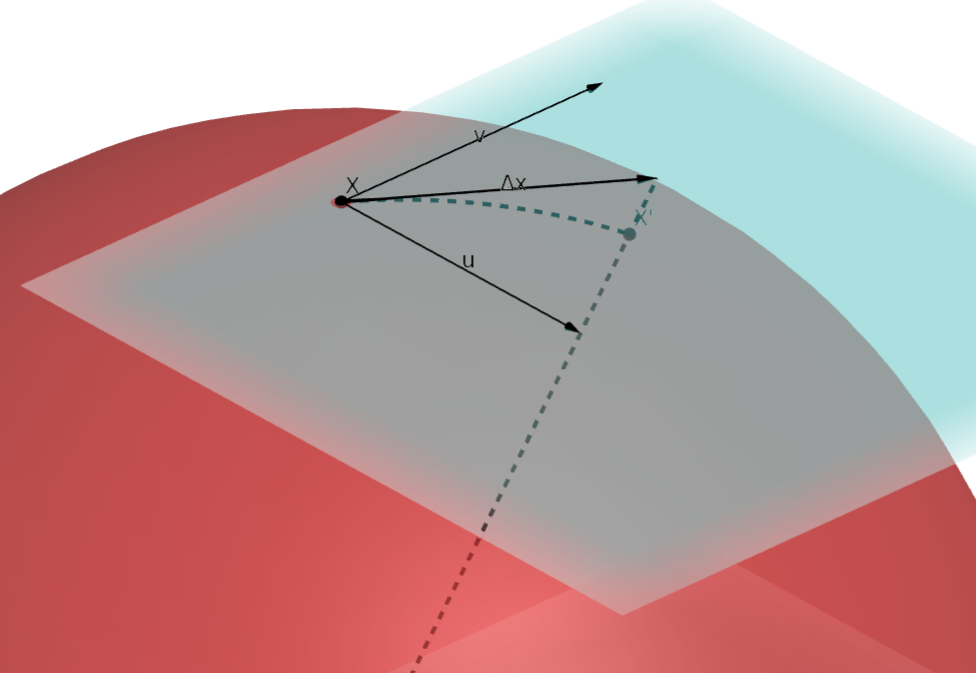
\includegraphics[height=0.7\textheight, keepaspectratio]{sphere-local.png}
    \caption*{Локальная параметризация на сфере}
  \end{figure}
\end{frame}

\begin{frame}
  \frametitle{Локальные параметризации}
  \framesubtitle{Общая теория}
  Пусть $\mathbf{r}: M\to\mathbb{R}^n$, $M\subset \mathbb{R}^m$ --- $k$-мерное многообразие, $\mathbf{x}_0\in \mathbb{R}^m$.

  $\varphi_{\mathbf{x}_0}:U\to \mathbb{R}^k$ --- \emph{карта} многообразия в окрестности $U\subset M$ точки $\mathbf{x}_0$.
 
  Тогда мы можем на каждом шаге ЛМ подменять функцию остатков на $\mathbf{\tilde{r}}$
  $$ \mathbf{\tilde{r}}\left(\mathbf{x}\right)=\mathbf{r}\left(\varphi_{\mathbf{x}_0}^{-1}\left(\Delta\mathbf{x}\right)\right)$$

  При этом доверительный регион оказывается в $\mathbb{R}^k$, якобиан функции остатков изменяется по цепному правилу $\mathbf{\tilde{J}}=\mathbf{J}\dd{\varphi_{\mathbf{x}_0}^{-1}}$
\vspace{0.7cm}

  Часто встречается нотация $\mathbf{x}_0\boxplus\Delta\mathbf{x}=\varphi_{\mathbf{x}_0}^{-1}\left(\Delta\mathbf{x}\right)$.
\end{frame}

\begin{frame}
  \frametitle{Локальные параметризации}
  \framesubtitle{Примеры}
  \begin{itemize}
    \item окружность $S^1$ ($\Delta x$ -- угол, на который мы вращаемся от $\left(x, y\right)^\intercal$)
      $$
      \begin{pmatrix}
        x \\
        y
      \end{pmatrix}
        \boxplus\Delta x=
      \begin{pmatrix}
        x\cos\left(\Delta x\right)-y\sin\left(\Delta x\right) \\
        x\sin\left(\Delta x\right)+y\cos\left(\Delta x\right)
      \end{pmatrix}
      $$
    \item $SO(3)$
      $$\mathbf{\mathbf{R}}\boxplus\Delta\mathbf{R}=\mathbf{R}\exp\left(\Delta\mathbf{R}\right)$$
    \item $SE(3)$ --- аналогично
  \end{itemize}
\end{frame}

\begin{frame}
  \frametitle{Отображение $\exp$ в $SO(3)$ и в $SE(3)$}
  \begin{itemize}
    \item $\omega\in \mathfrak{so}(3)$ задает ось вращения, $\left\Vert\omega\right\Vert$ --- угол вращения.
    \begin{equation*}
      \exp\left(\omega\right)=\exp\left(\omega_{\cross}\right)=\mathbf{I}+\left(\frac{\sin\left\Vert\omega\right\Vert}{\left\Vert\omega\right\Vert}\right)\omega_{\cross}+\left(\frac{1-\cos\left\Vert\omega\right\Vert}{\left\Vert\omega\right\Vert^2}\right)\omega_{\cross}^2
    \end{equation*}

  \item $\left(\omega; \mathbf{u}\right)\in \mathfrak{se}(3)$
    \begin{equation*}
    \begin{gathered}
      \mathbf{R}=\exp\left(\omega\right) \\
      \mathbf{V}=\mathbf{I}+\left(\frac{1-\cos\left\Vert\omega\right\Vert}{\left\Vert\omega\right\Vert^2}\right)\omega_{\cross}+\left(\frac{\left\Vert\omega\right\Vert-\sin\left\Vert\omega\right\Vert}{\left\Vert\omega\right\Vert^3}\right)\omega_{\cross}^2 \\
      \exp\left(\omega; \mathbf{u}\right)=\exp
      \begin{pmatrix}
        \begin{array}{c|c}
          \omega_{\cross} & \mathbf{u} \\
          \hline
          \mathbf{0}^\intercal & 0
        \end{array}
      \end{pmatrix} =
      \begin{pmatrix}
        \begin{array}{c|c}
          \mathbf{R} & \mathbf{V}\mathbf{u} \\
          \hline
          \mathbf{0}^\intercal & 1
        \end{array}
      \end{pmatrix}
    \end{gathered}
    \end{equation*}
  \end{itemize}
\end{frame}

\begin{frame}
  \frametitle{Функции потерь}
  \begin{figure}
    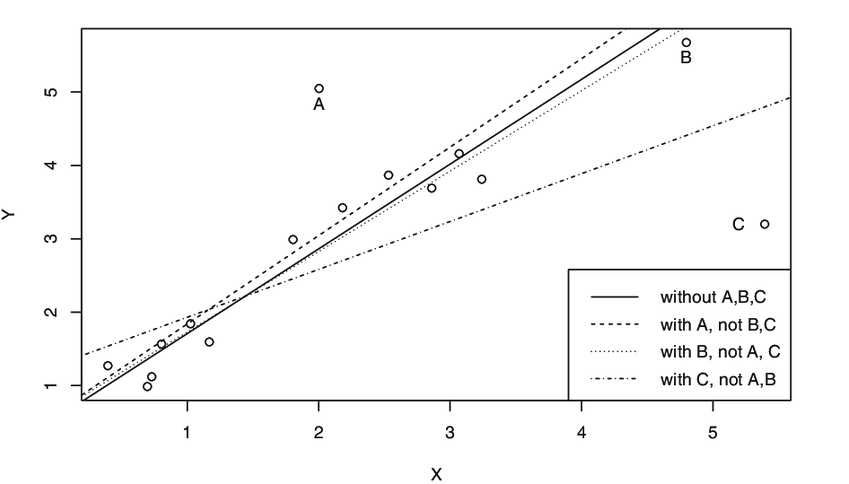
\includegraphics[height=0.7\textheight, keepaspectratio]{outliers.png}
    \caption*{Линейная регрессия при наличии аутлаеров}
  \end{figure}
\end{frame}

\begin{frame}
  \frametitle{Функции потерь}
  \begin{columns}[c]
    \begin{column}{0.5\textwidth}
      Обновим целевую функцию
      $$F\left(\mathbf{x}\right)=\frac{1}{2}\sum_{i=1}^n\rho\left(r_i^2\left(\mathbf{x}\right)\right)$$
      \begin{itemize}
        \item $\left|r_i\left(\mathbf{x}\right)\right|<r_{th} \implies \rho\left(r_i\left(\mathbf{x}\right)\right)\approx r_i^2\left(\mathbf{x}\right)$
        \item $\left|r_i\left(\mathbf{x}\right)\right|\gg r_{th} \implies \rho\left(r_i\left(\mathbf{x}\right)\right)\ll r_i^2\left(\mathbf{x}\right)$
      \end{itemize}
    \end{column}

    \begin{column}{0.5\textwidth}
      \begin{figure}
        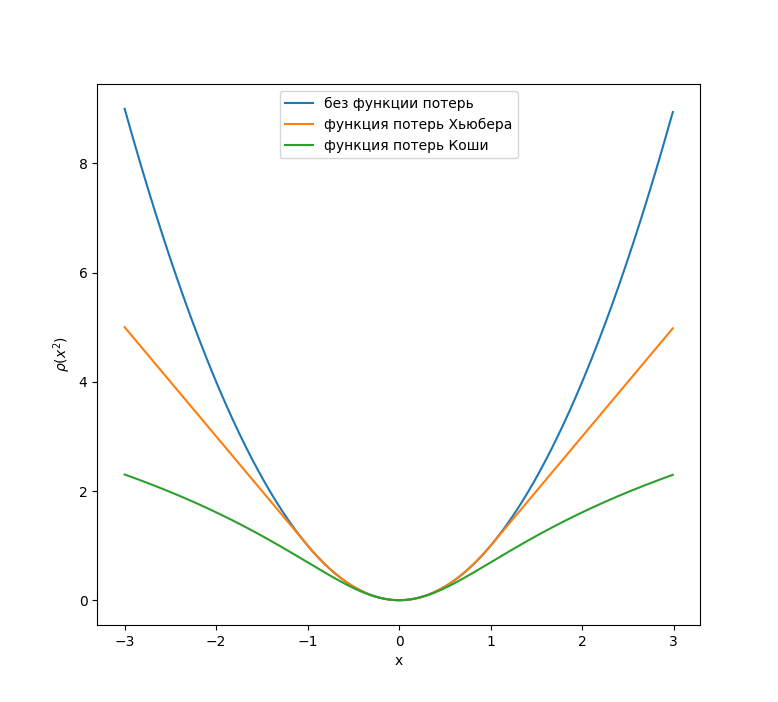
\includegraphics[height=0.7\textheight, keepaspectratio]{loss.png}
        \vspace{-0.5cm}
        \caption*{Примеры функций потерь $\rho\left(x^2\right)$}
      \end{figure}
    \end{column}
  \end{columns}
\end{frame}

\begin{frame}
  \frametitle{Функции потерь}
  \framesubtitle{Простая обработка}
  Перепишем новую целевую функцию
  $$F\left(\mathbf{x}\right)=\frac{1}{2}\sum_{i=1}^n\rho\left(r_i^2\left(\mathbf{x}\right)\right)=\frac{1}{2}\sum_{i=1}^n\left(\sqrt{\rho\left(r_i^2\left(\mathbf{x}\right)\right)}\right)^2=\frac{1}{2}\sum_{i=1}^n{\tilde{r}_i}^2\left(\mathbf{x}\right)$$
  Для новой функции остатков тривиально пересчитывается якобиан $\tilde{\mathbf{J}}=\mathbf{W}\mathbf{J}$, и получаются выражения для $\mathbf{H}$ и $\mathbf{g}$:
  $$\mathbf{H}=\mathbf{J}^\intercal \mathbf{W}^2\mathbf{J} \qquad \mathbf{g}=\mathbf{J}^\intercal\mathbf{W}\tilde{\mathbf{r}}$$
\end{frame}

\begin{frame}
  \frametitle{Функции потерь}
  \framesubtitle{Продвинутая обработка}
  Усложним целевую функцию еще немного
    $$F\left(\mathbf{x}\right)=\frac{1}{2}\sum_{i=1}^N\rho\left(\left\Vert\mathbf{r}_i\left(\mathbf{x}\right)\right\Vert^2\right) \quad \mathbf{r}_i\left(\mathbf{x}\right)\in\mathbb{R}^{n_i}$$
  Сконцентрируемся теперь на одном ее члене $G\left(\mathbf{x}\right)=\frac{1}{2}\rho\left(\left\Vert\mathbf{r}\left(\mathbf{x}\right)\right\Vert^2\right)$, $\mathbf{r}\left(\mathbf{x}\right)\in \mathbb{R}^n$.
    \begin{equation*}
      \begin{gathered}
        \pdv{G\left(\mathbf{x}\right)}{x_i}=\rho'\sum_{k=1}^n\pdv{r_k\left(\mathbf{x}\right)}{x_i}r_k\left(\mathbf{x}\right)
      \end{gathered}
    \end{equation*}
\end{frame}

\begin{frame}
  \frametitle{Функции потерь}
  \framesubtitle{Продвинутая обработка}

  \begin{equation*}
      \pdv{G\left(\mathbf{x}\right)}{x_i}=\rho'\sum_{k=1}^nr_k\left(\mathbf{x}\right)\pdv{r_k\left(\mathbf{x}\right)}{x_i}
  \end{equation*}
      {\begin{align}
        \pdv{G\left(\mathbf{x}\right)}{x_i}{x_j}
         & =2\rho''\left(\sum_{k=1}^nr_k\left(\mathbf{x}\right)\pdv{r_k\left(\mathbf{x}\right)}{x_i}\right)^2 \label{dd:1} \\
         & +\rho'\sum_{k=1}^n\pdv{r_k\left(\mathbf{x}\right)}{x_i}\pdv{r_k\left(\mathbf{x}\right)}{x_j} \label{dd:2} \\
         & +\rho'\sum_{k=1}^n\pdv{r_k\left(\mathbf{x}\right)}{x_i}{x_j}r_k\left(\mathbf{x}\right) \label{dd:3}
      \end{align}}
\end{frame}

\begin{frame}
  \frametitle{Функции потерь}
  \framesubtitle{Продвинутая обработка}
  \begin{itemize}
    \item без функции потерь $\implies$ $(\ref{dd:1})=0$, отбрасываем $(\ref{dd:3})$
    \item простая обработка $\implies$ отбрасываем и $(\ref{dd:1})$, и $(\ref{dd:3})$ 
    \item продвинутая обработка $\implies$ отбрасываем только $(\ref{dd:3})$
  \end{itemize}

  В последнем случае имеем
  $$\mathbf{H}=\mathbf{J}^\intercal\left(\rho'\mathbf{I}+2\rho''\mathbf{r}\mathbf{r}^\intercal\right)\mathbf{J} \qquad \mathbf{g}=\rho'\mathbf{J}^\intercal\tilde{\mathbf{r}}$$
\end{frame}

\begin{frame}
  \frametitle{Функции потерь}
  \framesubtitle{Продвинутая обработка}
  Оказывается, мы снова можем ``подменить задачу'', выбрав новые $\tilde{\mathbf{J}}$ и $\tilde{\mathbf{g}}$. 

  Пусть $\alpha$ --- корень уравнения 
  $$\frac{1}{2}\alpha^2-\alpha-\frac{\rho''}{\rho'}\left\Vert\mathbf{r}\right\Vert^2=0$$

  Тогда положим
  \begin{equation*}
    \begin{gathered}
      \tilde{\mathbf{r}}=\frac{\sqrt{\rho'}}{1-\alpha}\mathbf{r} \\
      \tilde{\mathbf{J}}=\sqrt{\rho'}\left(\mathbf{I}-\alpha\frac{\mathbf{r}\mathbf{r}^\intercal}{\left\Vert\mathbf{r}\right\Vert^2}\right)\mathbf{J}
    \end{gathered}
  \end{equation*}

  В плохом случае, когда $2\rho''\left\Vert\mathbf{r}\right\Vert^2+\rho'<0$, можем положить $\alpha=1-\varepsilon$ --- так мы хотя бы частично учтём функцию потерь.
\end{frame}

\begin{frame}
  \frametitle{Структура разреженности $H$}
  Чтобы эффективно находить $\argmin\left\Vert\mathbf{J}\mathbf{x}-\mathbf{r}\right\Vert$, мы хотим понять, на каких клетках $\mathbf{J}$ и $\mathbf{H}$ могут принимать ненулевые значения.
  \begin{itemize}
    \item $\mathbf{J}_{i,j}\neq 0$ $\implies$ $i$-й остаток существенно зависит от $j$-го параметра
    \item $\mathbf{H}_{j_1,j_2}\neq 0$ $\implies$ $j_1$-й и $j_2$-й параметры присутствуют вместе в некотором остатке.
 \end{itemize}
\end{frame}

\begin{frame}
  \frametitle{Структура разреженности $H$}
  \begin{figure}
    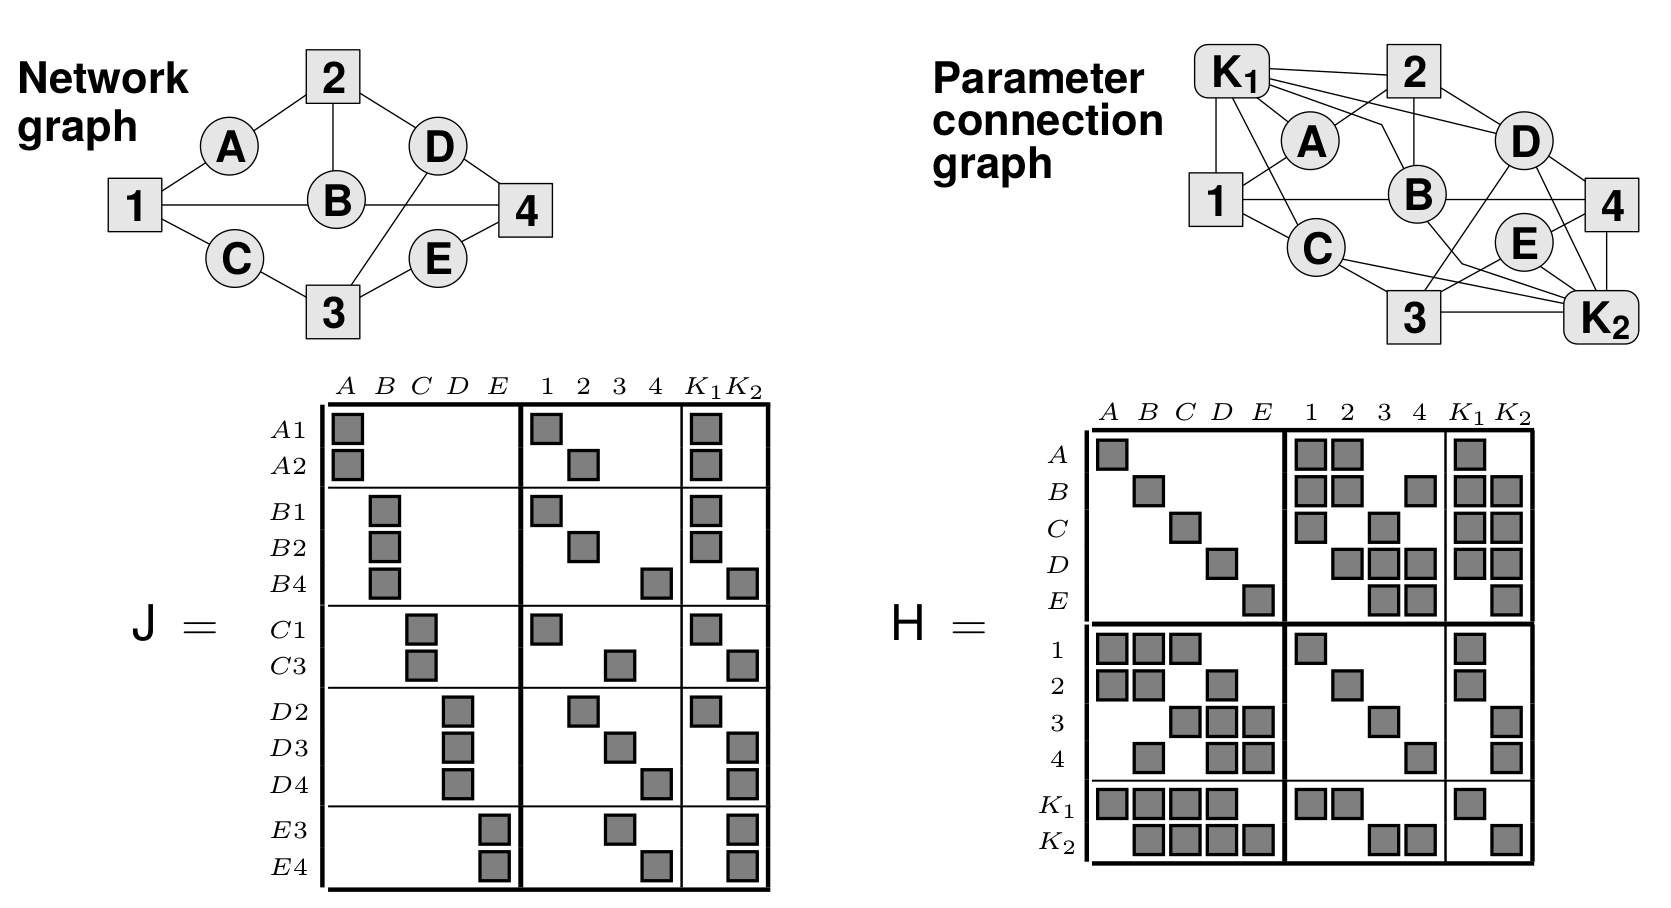
\includegraphics[height=0.7\textheight, keepaspectratio]{h-struct.png}
    \caption*{1-4 --- кадры; A-E --- наблюдаемые точки; K1, K2 --- параметры камер}
  \end{figure}
\end{frame}

\begin{frame}
  \frametitle{Структура разреженности $H$}
  \framesubtitle{Дополнение Шура}
  \begin{columns}
    \begin{column}{0.5\textwidth}
      Предположим, что мы решаем задачу SfM и пытаемся определить положения камер и ключевых точек. В простейшем случае $\mathbf{H}$ имеет вид
      $$
      \mathbf{H}=
      \begin{pmatrix}
        \begin{array}{c|c}
          \mathbf{H}_{cc} & \mathbf{H}_{cp} \\
          \hline
          \mathbf{H}_{cp}^\intercal & \mathbf{H}_{pp}
        \end{array}
      \end{pmatrix}
      $$

    \end{column}
    \begin{column}{0.5\textwidth}
      \begin{figure}
        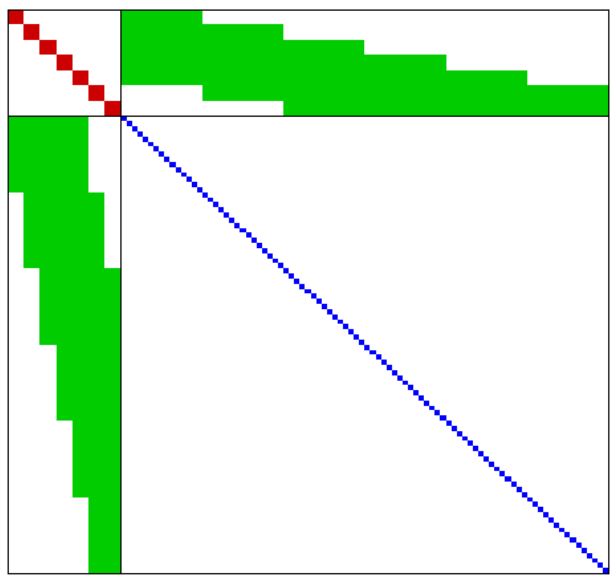
\includegraphics[height=0.7\textheight, keepaspectratio]{h-struct-easy.png}
        \caption*{Структура рассматриваемой $\mathbf{H}$}
      \end{figure}
    \end{column}
  \end{columns}
\end{frame}

\begin{frame}
  \frametitle{Структура разреженности $H$}
  \framesubtitle{Дополнение Шура}
  Мы можем воспользоваться тем, что $\mathbf{H}_{pp}$ легко обратить\footnote[frame]{На самом деле легко решать системы вида $\mathbf{H}_{pp}\mathbf{x}=\mathbf{b}$}.
  $$
  \begin{cases}
    \mathbf{H}_{cc}\mathbf{x}_c+\mathbf{H}_{cp}\mathbf{x}_p=\mathbf{b}_c \\
    \mathbf{H}_{cp}^\intercal\mathbf{x}_c+\mathbf{H}_{pp}\mathbf{x}_p=\mathbf{b}_b
  \end{cases}
  $$
  \begin{equation*}
    \begin{gathered}
    \mathbf{x}_{p}=\mathbf{H}_{pp}^{-1}\mathbf{b}_p-\mathbf{H}_{pp}^{-1}\mathbf{H}_{cp}^\intercal\mathbf{x}_c \\
       \left(\mathbf{H}_{cc}-\mathbf{H}_{cp}\mathbf{H}_{pp}^{-1}\mathbf{H}_{cp}^\intercal\right)\mathbf{x}_c=\mathbf{b}_c-\mathbf{H}_{cp}\mathbf{H}_{pp}^{-1}\mathbf{b}_p \\
    \end{gathered}
  \end{equation*}
\end{frame}

\begin{frame}
  \frametitle{Оценки наибольшего правдоподобия}
  \framesubtitle{Выбор весов остатков}
  Пусть мы проводим $n$ измерений неизвестной величины $x\in\mathbb{R}$ с ошибками $\varepsilon_i\sim\mathcal{N}\left(0,\sigma_i^2\right)$ и получаем значения $x_i=x+\varepsilon_i$.
  
  Если бы мы знали $x$, плотность вероятности получения именно $\left\{x_i\right\}$ вычислялась бы как
  $$p\left(\left.\left\{x_i\right\}\right\rvert x\right)=\prod_{i=1}^n\frac{1}{2\sigma_i\sqrt{2\pi}}\exp\left\{-\frac{\left(x-x_i\right)^2}{2\sigma_i^2}\right\}$$

  Будем искать $\overline{x}$, который её максимизирует

  \begin{align*}
    \overline{x} & =\argmax_{x}p\left(\left.\left\{x_i\right\}\right\rvert x\right) \\
                 & =\argmin_{x}\sum_{i=1}^n\frac{\left(x_i-x\right)^2}{\sigma_i^2} \\
  \end{align*}
  
\end{frame}

\begin{frame}
  \frametitle{Оценки наибольшего правдоподобия}
  \framesubtitle{Функции потерь}
  Но что делать, если ошибки распределены по-другому?

  Пусть, например, $\varepsilon_i$ подчинены распределению Коши.

  \begin{align*}
    \overline{x} & =\argmax_{x}\prod_{i=1}^n\frac{1}{\pi \left(x_i-x\right)^2} \\
                 & =\argmin_{x}\sum_{i=1}^n \log\left(1+\left(x_i-x\right)^2\right) \\
  \end{align*}
  
  Мы получили оценку, соответствующую функции потерь Коши.
\end{frame}

\begin{frame}
  \frametitle{Оценки наибольшего правдоподобия}
  \framesubtitle{Теорема Гаусса-Маркова}
  Теперь будем наблюдать линейную регрессию 
  $$\mathbf{y}=\mathbf{X}\boldsymbol{\beta}+\boldsymbol{\varepsilon}_i$$
  где $\mathbf{y}\in\mathbb{R}^n, \mathbf{X}\in\mathbb{R}^{n\cross m}, \boldsymbol{\beta}\in\mathbb{R}^m, \boldsymbol{\varepsilon}_i\sim\mathcal{N}\left(\mathbf{0},\sigma \mathbf{I}\right)$.

  Оказывается, при условиях

  \begin{itemize}
    \item $\mathrm{E}\left[\boldsymbol{\varepsilon_i}\right]=\mathbf{0}$ --- \emph{несмещенность ошибок}
    \item $\mathrm{D}\left[\boldsymbol{\varepsilon_i}\right]=\mathrm{D}\left[\boldsymbol{\varepsilon_j}\right]$ --- \emph{гомоскедакстичность}
   \item $\mathrm{Cov}\left[\boldsymbol{\varepsilon_i},\boldsymbol{\varepsilon_j}\right]=\mathbf{0}$ --- \emph{некоррелированность ошибок}
  \end{itemize}

  $\overline{\boldsymbol{\beta}}=\argmax{\left\Vert\mathbf{X}\boldsymbol{\beta}-\mathbf{y}\right\Vert}$ является оценкой наибольшего правдоподобия!
\end{frame}

\begin{frame}
  \frametitle{Применение на практике: ceres-solver}
  \lstinputlisting[language=C++, basicstyle=\tiny]{example.cpp}
\end{frame}

\begin{frame}
  \frametitle{Применение на практике: ceres-solver}
  \begin{columns}
    \begin{column}{0.4\textwidth}
      \begin{equation*}
        r\left(x, y\right)\approx
        \begin{pmatrix}
          \sqrt{x}-1.41 \\
          y-2
        \end{pmatrix}
      \end{equation*}
      При этом $\sqrt{x}$ находится численным методом Ньютона. Несмотря на это, ceres-solver способен продифференцировать \emph{программу}, вычисляющую $r$ и найти $\argmin\left\Vert r\right\Vert^2$.
    \end{column}

    \begin{column}{0.6\textwidth}
      \begin{figure}
        \begin{tikzpicture}
        \begin{axis}[
            title={$\frac{1}{2}\left\Vert r\left(x, y\right)\right\Vert^2$}, 
            xlabel=$x$, ylabel=$y$,
                small,
        ]
        \addplot3[
                surf,
                domain=1:3,
                domain y=1:3,
        ] 
                {0.5 * ((sqrt(x) - 1.41) ^ 2 + (1 / 9) * (y - 2) ^ 2)};
        \end{axis}
        \end{tikzpicture}
      \end{figure}
    \end{column}
  \end{columns}
\end{frame}

\end{document}
